\documentclass[12pt, a4paper]{article}

% Codificacao e idioma
\usepackage[utf8]{inputenc}
\usepackage[T1]{fontenc}
\usepackage[brazilian]{babel}

% Layout e margem ABNT
\usepackage[top=3cm, bottom=2cm, left=3cm, right=2cm]{geometry}

% Tipografia
\usepackage{times}
\usepackage{setspace}
\onehalfspacing

% Figuras e tabelas
\usepackage{graphicx}
\usepackage{float}
\usepackage{booktabs}
\usepackage{longtable}
\usepackage{array}
\usepackage{tabularx}

% Codigos e cores
\usepackage{listings}
\usepackage{xcolor}

% Posicionamento absoluto
\usepackage{tikz}

% Links e referencias
\usepackage[hidelinks]{hyperref}
\usepackage{csquotes}
\usepackage[
  backend=biber,
  style=abnt,
  citestyle=abnt
]{biblatex}
\addbibresource{referencias.bib}

% Identacao do primeiro paragrafo
\usepackage{indentfirst}

% Titulos de secao
\setcounter{secnumdepth}{3}
\setcounter{tocdepth}{3}

% Configuracao de listings
\lstset{
  basicstyle=\ttfamily\small,
  breaklines=true,
  frame=single,
  backgroundcolor=\color{gray!10},
  captionpos=b
}

\newcommand{\statusok}{\textbf{concluido}}
\newcommand{\statuspending}{\textbf{pendente}}
\newcommand{\RQ}[1]{\textbf{RQ#1}}

% -----------------------------------------------------------
\begin{document}
\pagenumbering{gobble}

% -----------------------------------------------------------
% CAPA
% -----------------------------------------------------------
\begin{titlepage}
\newgeometry{top=2cm, bottom=2cm, left=2.5cm, right=2.5cm}

\begin{tikzpicture}[remember picture, overlay]
  \node[anchor=north west, xshift=2.5cm, yshift=-2cm]
    at (current page.north west)
    {
\includegraphics[height=2.8cm]{figuras/brasao-unisantos.png}};
\end{tikzpicture}

\vspace*{1.2cm}

\begin{center}
  {\large\bfseries UNIVERSIDADE CAT\'OLICA DE SANTOS}\\[0.3cm]
  {\large Ci\^encia da Computa\c{c}\~ao}\\[0.3cm]
  {\large Inicia\c{c}\~ao Cient\'ifica}
\end{center}

\vfill

\begin{center}
  {\fontsize{25}{31}\selectfont\bfseries Quantiza\c{c}\~ao e Pruning em Opera\c{c}\~oes de Transformers}\\[0.55cm]
  {\large\bfseries Valida\c{c}\~ao Conceitual e Benchmarks Controlados em GPU}
\end{center}

\vfill\vfill

\begin{flushleft}
{\large
  Lucas Cerqueira Galv\~ao\\[0.25cm]
  Orientador: Prof. Me. Walter Silva Oliveira
}
\end{flushleft}

\vspace{1.8cm}

\begin{center}
  {\large Santos -- SP, setembro de 2026}
\end{center}

\restoregeometry
\end{titlepage}

\thispagestyle{empty}
\pagenumbering{roman}
\tableofcontents
\newpage
\pagenumbering{arabic}

% -----------------------------------------------------------
\section{Resumo}
% -----------------------------------------------------------

Este trabalho investiga em quais condi\c{c}\~oes t\'ecnicas compress\~ao
num\'erica e estrutural em Transformers se convertem em benef\'icios f\'isicos
reais de mem\'oria e desempenho durante infer\^encia. O estudo separa altera\c{c}\~ao
num\'erica, compress\~ao f\'isica e acelera\c{c}\~ao f\'isica, evitando tratar
zeros l\'ogicos, pesos compactos e kernels acelerados como a mesma evid\^encia.
Foram aprovadas 18 compara\c{c}\~oes conceituais entre implementa\c{c}\~ao manual,
NumPy, PyTorch, PyTorch SDPA e Keras/TensorFlow. Em seguida, foram executados
2.340 registros sint\'eticos, 117.000 amostras individuais de lat\^encia,
benchmarks f\'isicos com kernels INT8 e 2:4 confirmados, microbenchmarks de
crossover, avalia\c{c}\~oes OPT de 125M a 6.7B, an\'alise de sensibilidade por
componente/camada e uma tentativa h\'ibrida controlada. Os resultados mostram
que INT8 fake preservou melhor a sa\'ida que pruning no recorte sint\'etico; que
weight-only comprimiu mem\'oria e armazenamento preservando qualidade, mas sem
acelera\c{c}\~ao no backend avaliado; que INT8 dynamic e 2:4 s\'o sustentam
conclus\~oes f\'isicas quando representa\c{c}\~ao e kernel s\~ao confirmados; e que
speedups observados em modelos maiores podem ser inviabilizados por degrada\c{c}\~ao
de perplexidade. Nas configura\c{c}\~oes h\'ibridas, a seletividade por componente
preservou qualidade no OPT-1.3B, mas n\~ao se transferiu ao OPT-6.7B. Assim,
n\~ao foi demonstrada uma configura\c{c}\~ao que combinasse simultaneamente
preserva\c{c}\~ao de qualidade e speedup confirmado no maior modelo avaliado.

\noindent\textbf{Palavras-chave:} Transformer; self-attention; quantiza\c{c}\~ao; pruning; benchmark; inferencia.

\newpage

% -----------------------------------------------------------
\section{Introdu\c{c}\~ao}
% -----------------------------------------------------------

Arquiteturas Transformer se tornaram a base de grande parte dos sistemas
modernos de inteligencia artificial, especialmente em modelos de linguagem e
tarefas sequenciais. O mecanismo de aten\c{c}\~ao introduzido por
\textcite{vaswani2017attention} substituiu recorrencia explicita por opera\c{c}\~oes
matriciais altamente paralelizaveis, mas tambem concentrou custo em
proje\c{c}\~oes lineares densas, produto escalar entre consultas e chaves,
normaliza\c{c}\~ao softmax e combina\c{c}\~ao ponderada dos valores.

Esse custo e particularmente relevante durante inferencia, quando o objetivo
nao e treinar o modelo, mas executar previs\~oes de forma eficiente e
reprodutivel. Tecnicas como pruning e quantiza\c{c}\~ao prometem reduzir custo,
memoria e armazenamento. O problema e que nem toda redu\c{c}\~ao matematica ou
logica se transforma automaticamente em ganho fisico: zeros em uma matriz densa
podem continuar sendo multiplicados, e tensores dequantizados para ponto
flutuante podem preservar fidelidade sem executar aritmetica inteira
\cite{han2015learning,jacob2018quantization,dettmers2022llmint8}.

Esta inicia\c{c}\~ao cientifica parte dessa distin\c{c}\~ao. O objetivo nao e
somente comparar resultados numericos, mas classificar que tipo de evidencia
cada experimento realmente sustenta. Assim, uma valida\c{c}\~ao conceitual pode
mostrar que duas implementa\c{c}\~oes calculam a mesma opera\c{c}\~ao; um
benchmark sintetico pode mostrar robustez entre seeds e formatos de entrada; e
um experimento fisico precisa confirmar representa\c{c}\~ao, kernel e ambiente
antes de sustentar uma alega\c{c}\~ao de desempenho.

\subsection{Problema}

O problema investigado e: em opera\c{c}\~oes centrais de Transformers, quais
compromissos entre fidelidade numerica, armazenamento, memoria e latencia sao
observados ao aplicar pruning e quantiza\c{c}\~ao em inferencia?

Esse problema foi delimitado em dois objetos experimentais:

\begin{itemize}
  \item \textbf{proje\c{c}\~ao densa}, usada como controle das opera\c{c}\~oes
  lineares Q, K, V e O;
  \item \textbf{self-attention multi-head}, composta por proje\c{c}\~oes Q, K,
  V, separa\c{c}\~ao em cabe\c{c}as, scaled dot-product attention,
  recombina\c{c}\~ao e proje\c{c}\~ao de saida.
\end{itemize}

\subsection{Objetivo}

O objetivo geral e avaliar, em cenarios controlados de inferencia, os efeitos
de pruning e quantiza\c{c}\~ao sobre opera\c{c}\~oes de Transformers. Os
objetivos especificos sao:

\begin{itemize}
  \item validar conceitualmente a implementa\c{c}\~ao de self-attention;
  \item comparar implementa\c{c}\~oes independentes e bibliotecas consolidadas;
  \item medir fidelidade numerica entre baseline, pruning e quantiza\c{c}\~ao;
  \item verificar se os efeitos persistem entre seeds, perfis e distribui\c{c}\~oes;
  \item distinguir evidencias logicas de evidencias fisicas de hardware;
  \item repetir a analise em modelos OPT pre-treinados.
\end{itemize}

% -----------------------------------------------------------
\section{Fundamenta\c{c}\~ao}
% -----------------------------------------------------------

\subsection{Self-attention}

Na scaled dot-product attention, uma entrada e projetada em consultas
(\(Q\)), chaves (\(K\)) e valores (\(V\)). A matriz \(QK^T\) mede similaridade
entre posi\c{c}\~oes, e a divis\~ao por \(\sqrt{d_k}\) estabiliza a escala dos
logits antes da softmax. A saida e calculada pela combina\c{c}\~ao ponderada de
\(V\). Em multi-head attention, esse procedimento e executado em cabe\c{c}as
paralelas, concatenado e projetado novamente.

No estudo, a aten\c{c}\~ao multi-head e tratada como objeto principal porque
representa o bloco conceitual efetivamente usado em Transformers. A proje\c{c}\~ao
densa permanece no experimento por ser o componente linear compartilhado por
Q, K, V e O.

\subsection{Pruning}

Pruning remove ou zera parametros considerados menos relevantes. O pruning por
magnitude usa o valor absoluto dos pesos como criterio simples: pesos com menor
magnitude sao removidos primeiro \cite{han2015learning}. Neste trabalho, o
pruning denso e usado nos cenarios conceituais e sinteticos para observar erro
numerico. O pruning semiestruturado 2:4 e usado nos cenarios fisicos porque
pode acionar kernels especificos em hardware NVIDIA via cuSPARSELt
\cite{cusparselt2026}.

\subsection{Quantiza\c{c}\~ao}

Quantiza\c{c}\~ao reduz a precis\~ao numerica dos tensores. A forma fake INT8
simetrica por linha quantiza e dequantiza os pesos, preservando execu\c{c}\~ao
em ponto flutuante para medir fidelidade. Ja os caminhos fisicos diferenciam
INT8 weight-only, que evidencia armazenamento compacto de pesos, e INT8
dinamico, que tambem quantiza ativa\c{c}\~oes e pode confirmar computa\c{c}\~ao
inteira no profiler \cite{jacob2018quantization,torchao2026}.

% -----------------------------------------------------------
\section{Metodologia}
% -----------------------------------------------------------

\subsection{Perguntas de pesquisa}

O protocolo experimental foi organizado pelas seguintes perguntas:

\begin{description}
  \item[\RQ{1}] Como pruning e quantiza\c{c}\~ao alteram a fidelidade da saida?
  \item[\RQ{2}] As tecnicas reduzem armazenamento ou memoria?
  \item[\RQ{3}] As tecnicas reduzem latencia em opera\c{c}\~oes isoladas?
  \item[\RQ{4}] O tipo de evidencia permite distinguir fidelidade, representa\c{c}\~ao e kernel fisico?
  \item[\RQ{5}] As tendencias persistem entre seeds, distribui\c{c}\~oes e perfis?
  \item[\RQ{6}] Como a degrada\c{c}\~ao varia com sparsity de 10\%, 25\%, 50\% e 75\%?
  \item[\RQ{7}] As tendencias aparecem tambem em modelos OPT pre-treinados?
  \item[\RQ{8}] Quais tecnicas reduzem armazenamento, memoria ou latencia usando caminhos fisicos compativeis?
\end{description}

\subsection{Contrato de evidencia}

Uma tendencia foi considerada sustentada quando ocorreu em pelo menos 80\% dos
casos pareados e o intervalo bootstrap de 95\% nao cruzou o efeito nulo. Foi
classificada como mista quando dependeu de seed, perfil ou opera\c{c}\~ao, e
como contradita quando a dire\c{c}\~ao oposta foi predominante e consistente.
Ganho fisico relevante exigiu speedup mediano de pelo menos 1,05x, intervalo de
95\% inteiramente acima de 1,0x e confirma\c{c}\~ao do kernel correto.

\subsection{Valida\c{c}\~ao conceitual}

Antes dos benchmarks, a implementa\c{c}\~ao foi comparada com referencias
independentes. Foram avaliadas 18 compara\c{c}\~oes envolvendo NumPy manual,
PyTorch manual, PyTorch SDPA e Keras/TensorFlow \cite{paszke2019pytorch,abadi2016tensorflow}.
Os casos incluem a aten\c{c}\~ao sem mascaramento, mascaramento aditivo,
proje\c{c}\~oes Q/K/V/O e multi-head attention com \(H \in \{1,4,8\}\). Todas
as compara\c{c}\~oes usaram entradas e pesos compartilhados, com tolerancias
\texttt{atol=1e-6} e \texttt{rtol=1e-5}.

\subsection{Benchmark sintetico}

O benchmark sintetico v3 variou seeds, formas de entrada, numero de cabe\c{c}as
e distribui\c{c}\~oes. Foram usados 13 perfis de entrada, cinco seeds, seis
cenarios e tres repeti\c{c}\~oes para duas opera\c{c}\~oes, totalizando 2.340
registros agregados e 117.000 amostras individuais de latencia.

\begin{table}[H]
\centering
\caption{Estrutura do benchmark sintetico v3}
\begin{tabular}{ll}
\toprule
\textbf{Dimensao} & \textbf{Configura\c{c}\~ao} \\
\midrule
Opera\c{c}\~oes & proje\c{c}\~ao densa e self-attention multi-head \\
Perfis & 13 combina\c{c}\~oes de batch, sequencia, dimens\~ao e cabe\c{c}as \\
Seeds & 11, 23, 42, 101 e 2026 \\
Cenarios & FP32, INT8 fake, pruning 10\%, 25\%, 50\% e 75\% \\
Medi\c{c}\~ao & 20 warm-ups e 50 medi\c{c}\~oes por registro \\
\bottomrule
\end{tabular}
\end{table}

\subsection{Benchmark fisico}

O benchmark fisico foi executado em Linux via Docker Desktop com backend WSL2,
imagem PyTorch 2.11, CUDA 12.8, TorchAO e cuSPARSELt. A GPU alvo foi uma NVIDIA
RTX 4070 Ti SUPER com compute capability 8.9. Antes das medi\c{c}\~oes, um
probe confirmou CUDA, Triton, convers\~ao 2:4, forward finito e operadores
registrados no profiler \cite{docker2026,cusparselt2026,torchao2026}.

Os cenarios fisicos foram:

\begin{itemize}
  \item baseline BF16 compilado;
  \item INT8 weight-only por linha;
  \item INT8 dinamico de ativa\c{c}\~oes e pesos;
  \item baseline FP16 compilado;
  \item pruning semiestruturado 2:4 em FP16.
\end{itemize}

% -----------------------------------------------------------
\section{Resultados}
% -----------------------------------------------------------

\subsection{Equivalencia conceitual}

As 18 compara\c{c}\~oes foram aprovadas. O maior erro absoluto registrado foi
\(4{,}76837158 \times 10^{-7}\), valor compativel com arredondamento de ponto
flutuante. Assim, a implementa\c{c}\~ao manual e as bibliotecas avaliadas
executam a mesma constru\c{c}\~ao computacional dentro das tolerancias definidas.
Essa conclus\~ao autoriza os benchmarks seguintes a compararem transforma\c{c}\~oes
de pruning e quantiza\c{c}\~ao sobre um objeto experimental conceitualmente
validado.

\subsection{Fidelidade no benchmark sintetico}

No recorte sintetico, a quantiza\c{c}\~ao fake por linha apresentou MSE menor
que pruning em 100\% dos casos pareados. A degrada\c{c}\~ao do pruning cresceu
monotonicamente com a sparsity, como esperado.

\begin{table}[H]
\centering
\caption{MSE medio por cenario no benchmark sintetico v3}
\begin{tabular}{lrr}
\toprule
\textbf{Cenario} & \textbf{Proje\c{c}\~ao densa} & \textbf{Multi-head attention} \\
\midrule
INT8 fake por linha & \(5{,}854\times10^{-5}\) & \(1{,}349\times10^{-5}\) \\
Pruning 10\% & \(5{,}676\times10^{-4}\) & \(1{,}285\times10^{-4}\) \\
Pruning 25\% & \(8{,}984\times10^{-3}\) & \(2{,}003\times10^{-3}\) \\
Pruning 50\% & \(7{,}669\times10^{-2}\) & \(1{,}425\times10^{-2}\) \\
Pruning 75\% & \(2{,}971\times10^{-1}\) & \(3{,}394\times10^{-2}\) \\
\bottomrule
\end{tabular}
\end{table}

\begin{figure}[H]
  \centering
  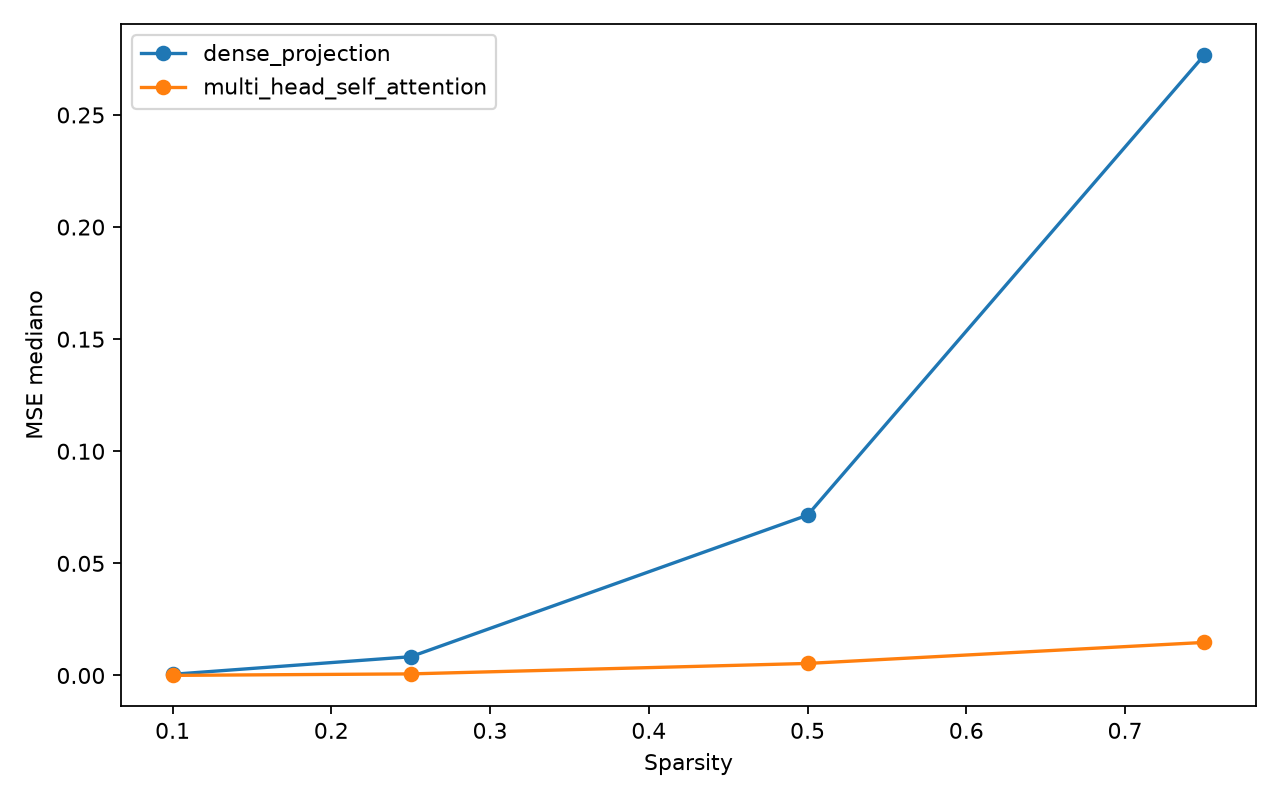
\includegraphics[width=0.82\textwidth]{figuras/sintetico_qualidade_por_sparsity.png}
  \caption{Degrada\c{c}\~ao numerica por nivel de sparsity no benchmark sintetico.}
\end{figure}

\subsection{Latencia no benchmark sintetico}

Os tempos do benchmark sintetico nao sustentam conclus\~ao de acelera\c{c}\~ao
fisica. As matrizes permanecem densas, a quantiza\c{c}\~ao fake retorna a FP32,
e nenhum kernel INT8 ou sparse e usado. Por isso, a bateria sintetica foi
interpretada como evidencia de fidelidade e robustez numerica, nao como prova
de desempenho em hardware.

\begin{figure}[H]
  \centering
  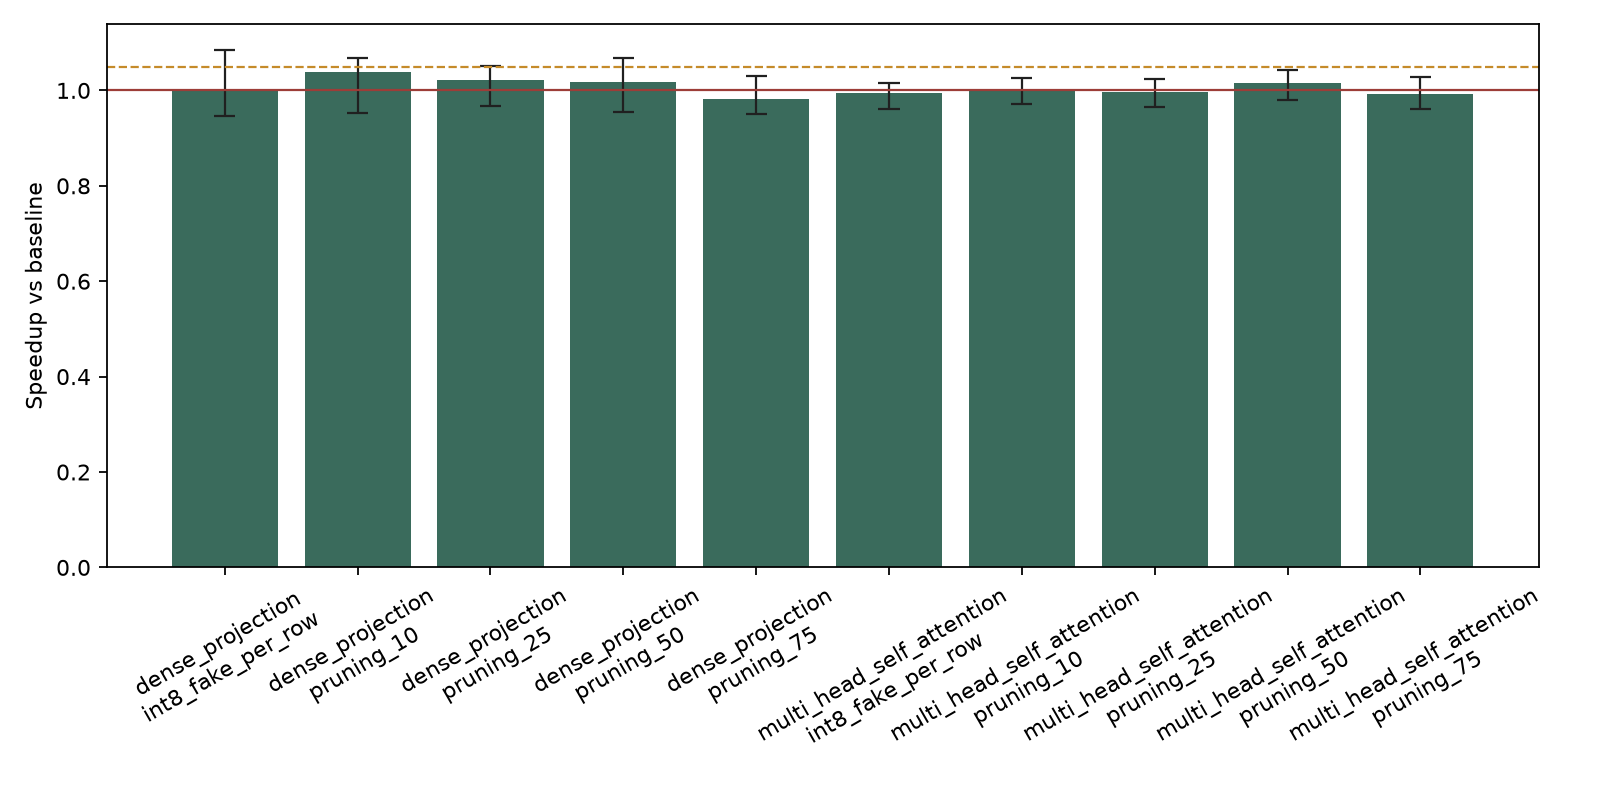
\includegraphics[width=0.82\textwidth]{figuras/sintetico_speedup_ci95.png}
  \caption{Speedup sintetico com intervalos bootstrap de 95\%; sem confirma\c{c}\~ao de kernel fisico.}
\end{figure}

\subsection{Resultados fisicos}

Na bateria fisica, todos os candidatos reduziram armazenamento e memoria de
pico mediana. No entanto, os seis grupos de desempenho tiveram speedup mediano
abaixo de 1,0x, com intervalos bootstrap inteiramente abaixo do baseline. Logo,
para estes shapes, esta GPU e esta implementa\c{c}\~ao, a hipotese de ganho de
latencia foi contradita.

\begin{table}[H]
\centering
\caption{Resumo fisico por opera\c{c}\~ao e cenario}
\resizebox{\textwidth}{!}{%
\begin{tabular}{llrrr}
\toprule
\textbf{Opera\c{c}\~ao} & \textbf{Cenario} & \textbf{Speedup mediano} & \textbf{Memoria mediana} & \textbf{Armazenamento} \\
\midrule
Proje\c{c}\~ao densa & INT8 dinamico & 0,808 & 0,801 & 0,504 \\
Proje\c{c}\~ao densa & INT8 weight-only & 0,136 & 0,801 & 0,504 \\
Proje\c{c}\~ao densa & pruning 2:4 & 0,823 & 0,825 & 0,564 \\
Multi-head attention & INT8 dinamico & 0,650 & 0,639 & 0,503 \\
Multi-head attention & INT8 weight-only & 0,097 & 0,639 & 0,503 \\
Multi-head attention & pruning 2:4 & 0,645 & 0,728 & 0,562 \\
\bottomrule
\end{tabular}% 
}
\end{table}

\begin{figure}[H]
  \centering
  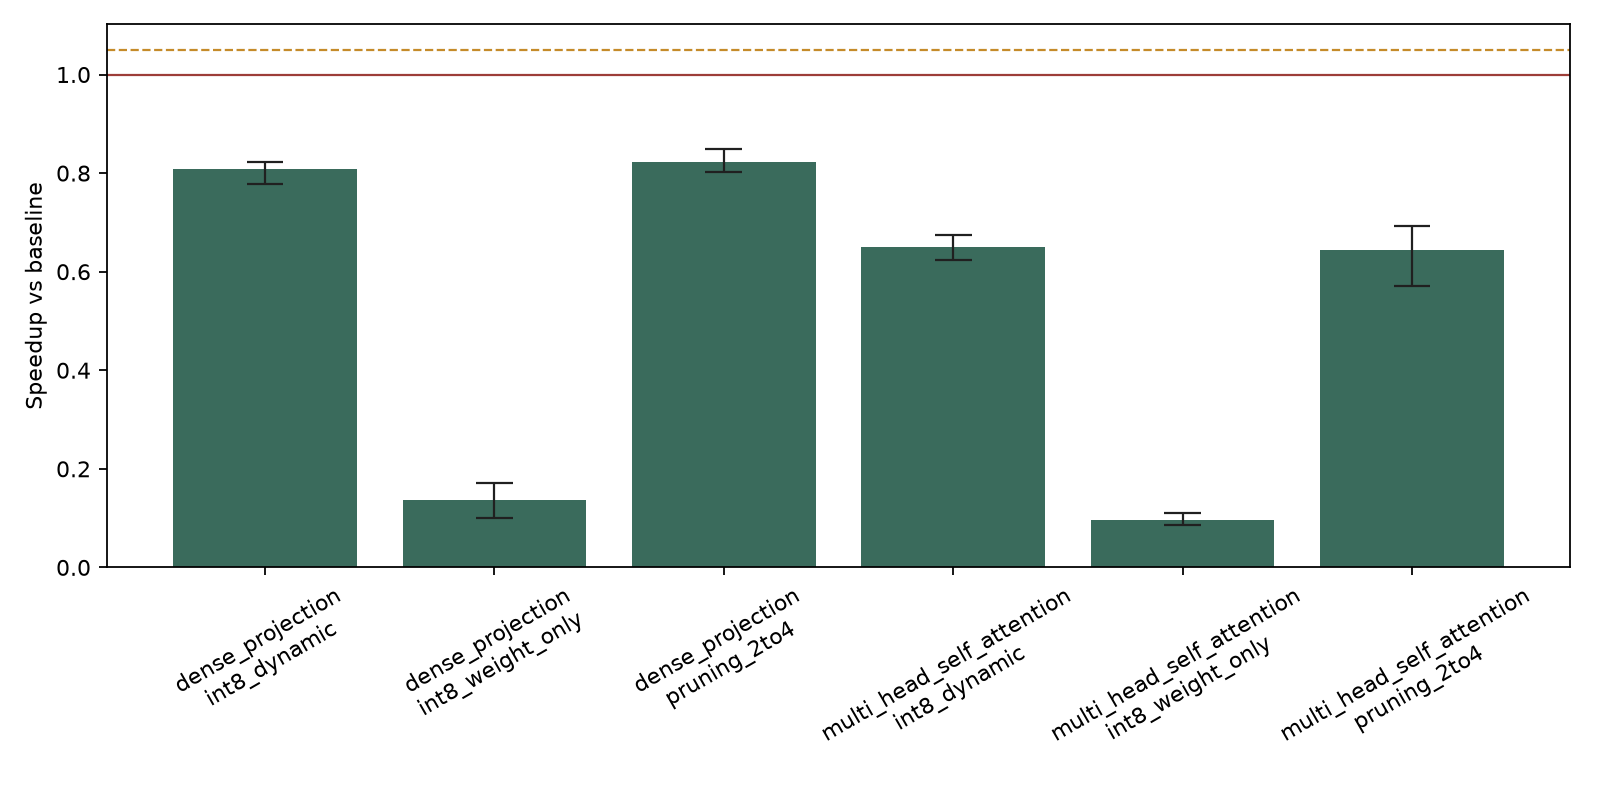
\includegraphics[width=0.88\textwidth]{figuras/hardware_speedup_ci95.png}
  \caption{Speedup fisico com intervalos bootstrap de 95\%; todos os grupos ficaram abaixo do baseline.}
\end{figure}

\begin{figure}[H]
  \centering
  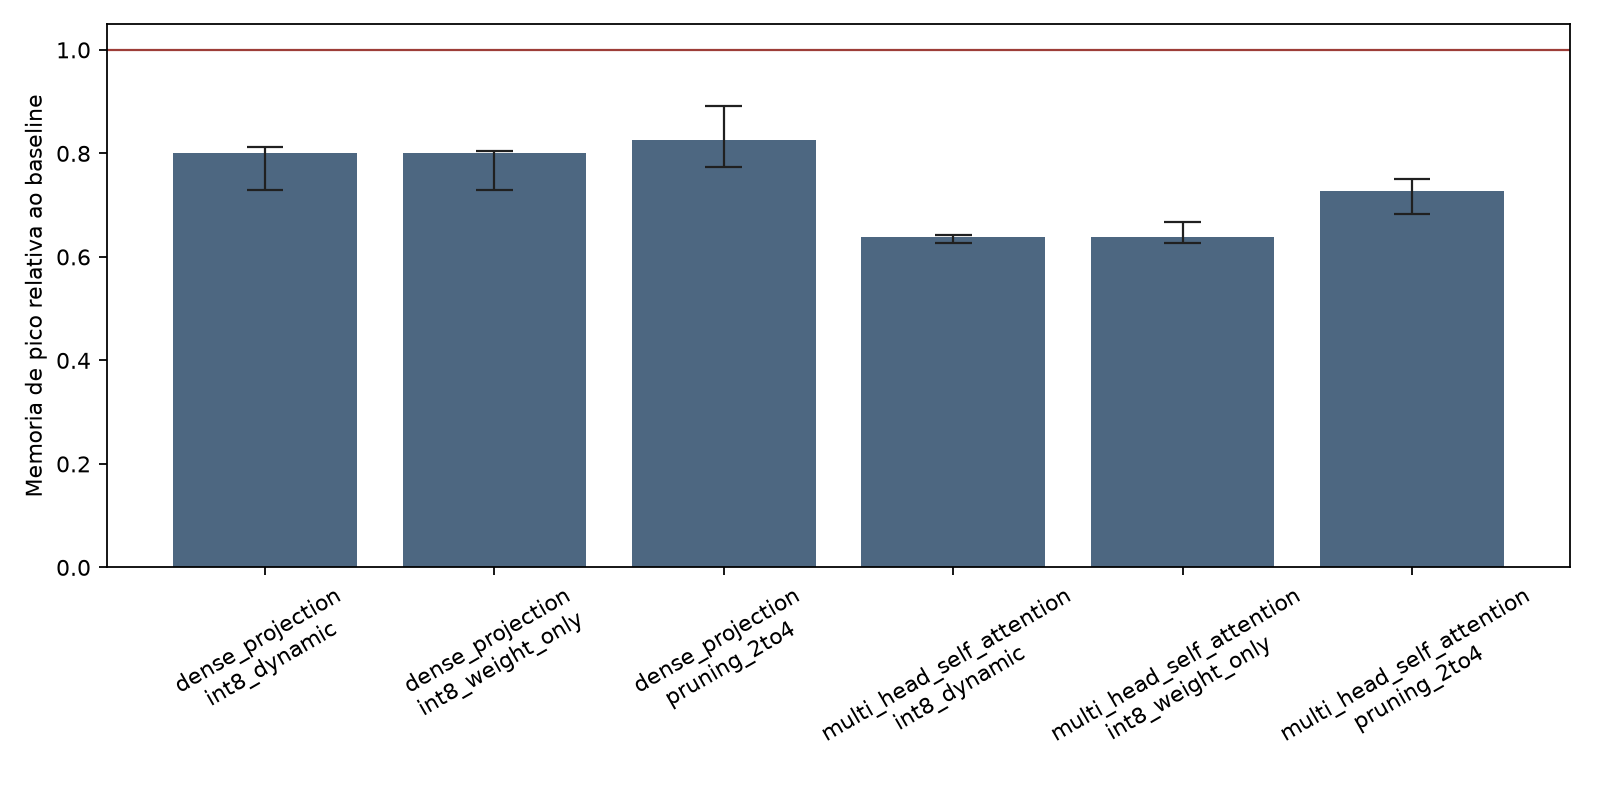
\includegraphics[width=0.88\textwidth]{figuras/hardware_memoria_pico_ci95.png}
  \caption{Memoria de pico relativa ao baseline nos cenarios fisicos.}
\end{figure}

\begin{figure}[H]
  \centering
  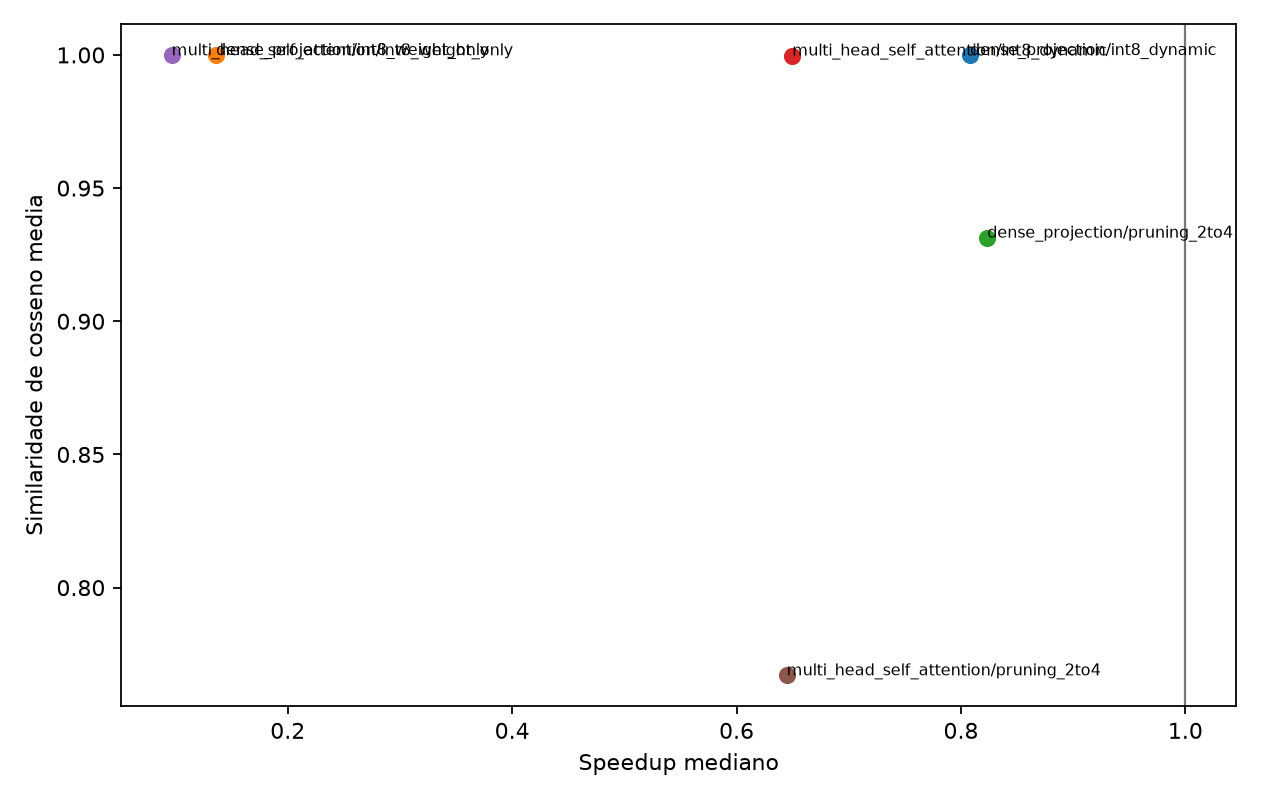
\includegraphics[width=0.82\textwidth]{figuras/hardware_pareto_qualidade_desempenho.png}
  \caption{Fronteira qualidade-desempenho para os cenarios fisicos avaliados.}
\end{figure}

\subsection{Modelos OPT pre-treinados}

Foram avaliados OPT-125M, OPT-350M e OPT-1.3B \cite{zhang2022opt}, sempre partindo das revisoes
originais e sem treinamento. A coleta usou 64 janelas de 512 tokens do
WikiText-2 e 20 prompts locais para comparar logits e geracao. A bateria
produziu 45 registros de qualidade, 2.880 janelas, 900 metricas de prompts,
1.296 registros de desempenho e 10.080 amostras individuais de timing.

\begin{table}[H]
\centering
\caption{Perplexidade dos modelos OPT em cenarios representativos}
\begin{tabular}{lrrr}
\toprule
\textbf{Modelo} & \textbf{Baseline BF16} & \textbf{INT8 fake atencao} & \textbf{Pruning 50\% atencao} \\
\midrule
OPT-125M & 42,371 & 42,313 & 65,796 \\
OPT-350M & 33,345 & 33,348 & 50,668 \\
OPT-1.3B & 21,394 & 21,384 & 28,644 \\
\bottomrule
\end{tabular}
\end{table}

Vinte e cinco das 45 variantes ficaram dentro dos limites operacionais. As
quantizacoes INT8 fake e weight-only foram estaveis nos tres modelos. O INT8
dinamico foi aceitavel em OPT-125M e OPT-350M, mas excedeu o limite em
OPT-1.3B. O pruning por magnitude em atencao foi aceitavel apenas em 10\%; a
partir de 25\%, a perplexidade ja excedeu o limite de 5\%.

\begin{figure}[H]
  \centering
  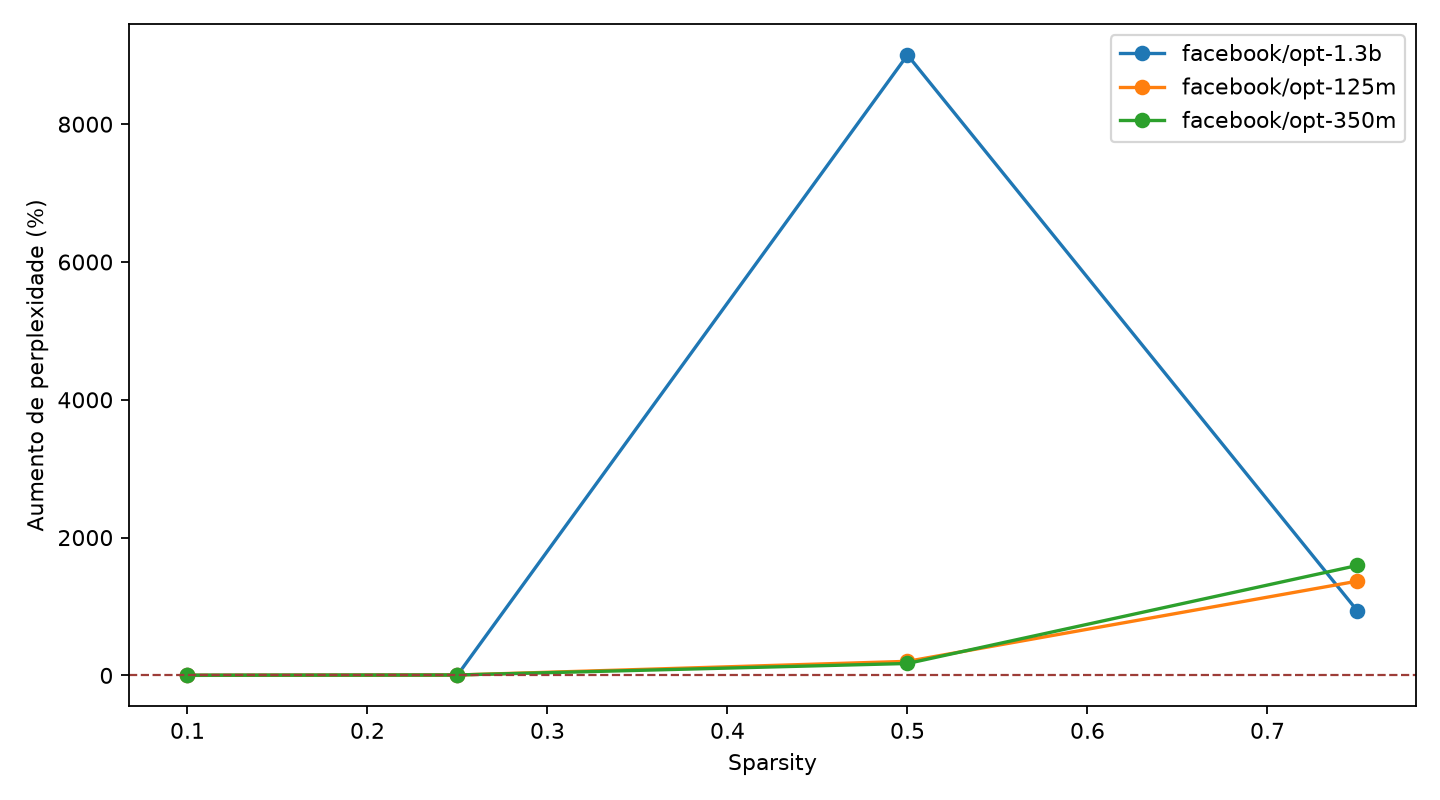
\includegraphics[width=0.88\textwidth]{figuras/opt_qualidade_por_sparsity_e_modelo.png}
  \caption{Perplexidade por sparsity e modelo na avaliacao OPT.}
\end{figure}

Em desempenho, prefill e TTFT foram medidos com registros completos. Nenhum
cenario cumpriu simultaneamente speedup mediano de pelo menos 1,05x, intervalo
de 95\% acima de 1,0x e kernel confirmado. O caso mais favoravel foi
\texttt{blocks\_int8\_dynamic} em OPT-1.3B, mas o intervalo de confianca ainda
cruzou o efeito nulo. Todos os casos planejados de decode foram preservados
como falha tecnica ou incompatibilidade: o problema observado foi a interacao
entre torch.compile, CUDA Graphs e atualizacao de KV cache.

\begin{figure}[H]
  \centering
  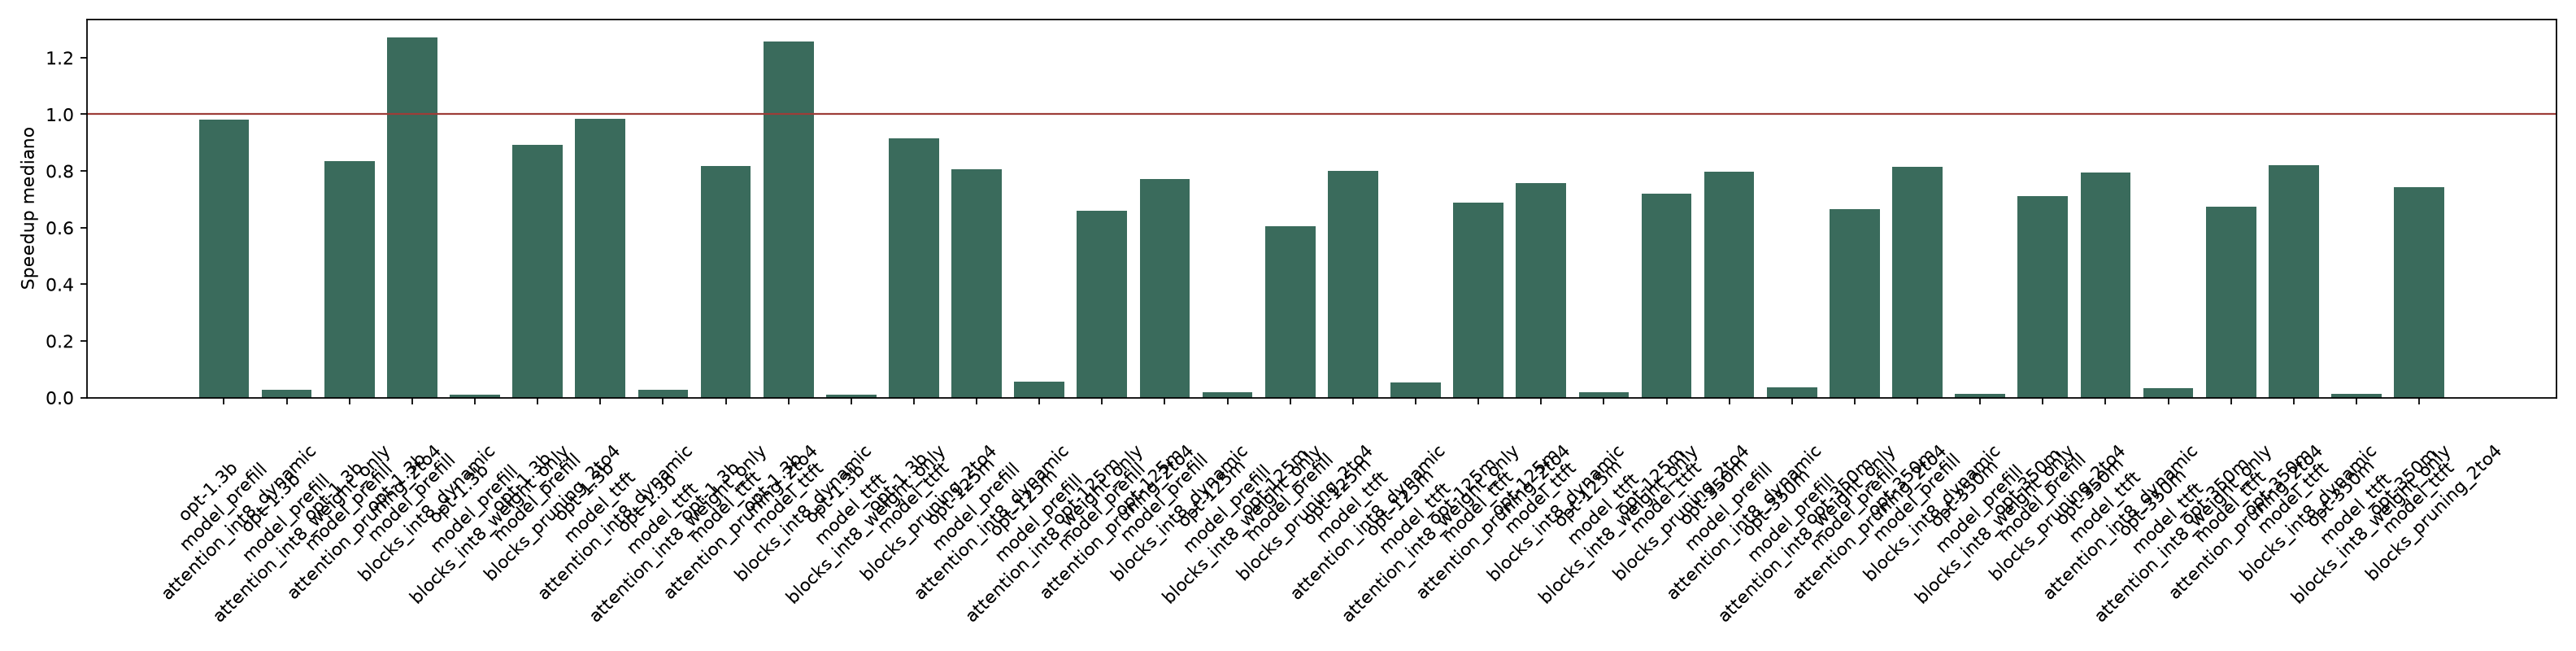
\includegraphics[width=0.88\textwidth]{figuras/opt_speedup_prefill_decode.png}
  \caption{Speedup em prefill e TTFT dos modelos OPT.}
\end{figure}

\subsection{Extensao de escala com OPT-2.7B e OPT-6.7B}

Apos a bateria principal, dois modelos maiores foram executados como extensao
exploratoria: OPT-2.7B e OPT-6.7B. Eles seguem o mesmo protocolo de qualidade e
desempenho, mas sao tratados separadamente para nao alterar os criterios
pre-registrados da bateria OPT v1. O objetivo foi verificar se o aumento de
parametros torna algum caminho fisico mais favoravel.

\begin{table}[H]
\centering
\caption{Qualidade e desempenho em modelos OPT maiores}
\resizebox{\textwidth}{!}{%
\begin{tabular}{llrrrr}
\toprule
\textbf{Modelo} & \textbf{Cenario} & \textbf{Perplexidade} &
\textbf{Aumento vs baseline} & \textbf{Speedup prefill} & \textbf{IC95 prefill} \\
\midrule
OPT-2.7B & baseline BF16 & 18,178 & 0,0\% & -- & -- \\
OPT-2.7B & atencao INT8 dinamico & 18,955 & 4,27\% & 1,024 & [0,844; 1,134] \\
OPT-2.7B & blocos INT8 dinamico & 18,981 & 4,42\% & 1,305 & [0,907; 1,588] \\
OPT-2.7B & atencao 2:4 & 27,670 & 52,22\% & 0,873 & [0,798; 0,907] \\
OPT-2.7B & blocos 2:4 & 519,074 & 2755,50\% & 1,061 & [0,975; 1,078] \\
\midrule
OPT-6.7B & baseline BF16 & 15,346 & 0,0\% & -- & -- \\
OPT-6.7B & atencao INT8 dinamico & 16,659 & 8,55\% & 1,169 & [1,009; 1,249] \\
OPT-6.7B & blocos INT8 dinamico & 40,675 & 165,05\% & 1,756 & [1,171; 2,137] \\
OPT-6.7B & atencao 2:4 & 21,311 & 38,87\% & 1,030 & [0,974; 1,111] \\
OPT-6.7B & blocos 2:4 & 168,097 & 995,38\% & 1,073 & [1,017; 1,228] \\
\bottomrule
\end{tabular}% 
}
\end{table}

O resultado muda a leitura da hipotese de escala. Em OPT-6.7B, o INT8 dinamico
aplicado aos blocos atingiu speedup mediano de 1,756 em prefill e 1,744 em
TTFT, com intervalos de 95\% acima de 1,0. Contudo, a perplexidade subiu de
15,346 para 40,675, aumento de 165\%. Portanto, ha ganho fisico, mas ele nao e
aceitavel pelo criterio operacional de qualidade. O mesmo vale para 2:4 aplicado
aos blocos: o speedup de prefill fica acima de 1,05 com intervalo acima de 1,0,
mas a perplexidade sobe para 168,097. A conclusao correta e que a escala pode
tornar alguns kernels mais rapidos, mas nao garante uma configuracao util se a
qualidade colapsar.

\begin{figure}[H]
  \centering
  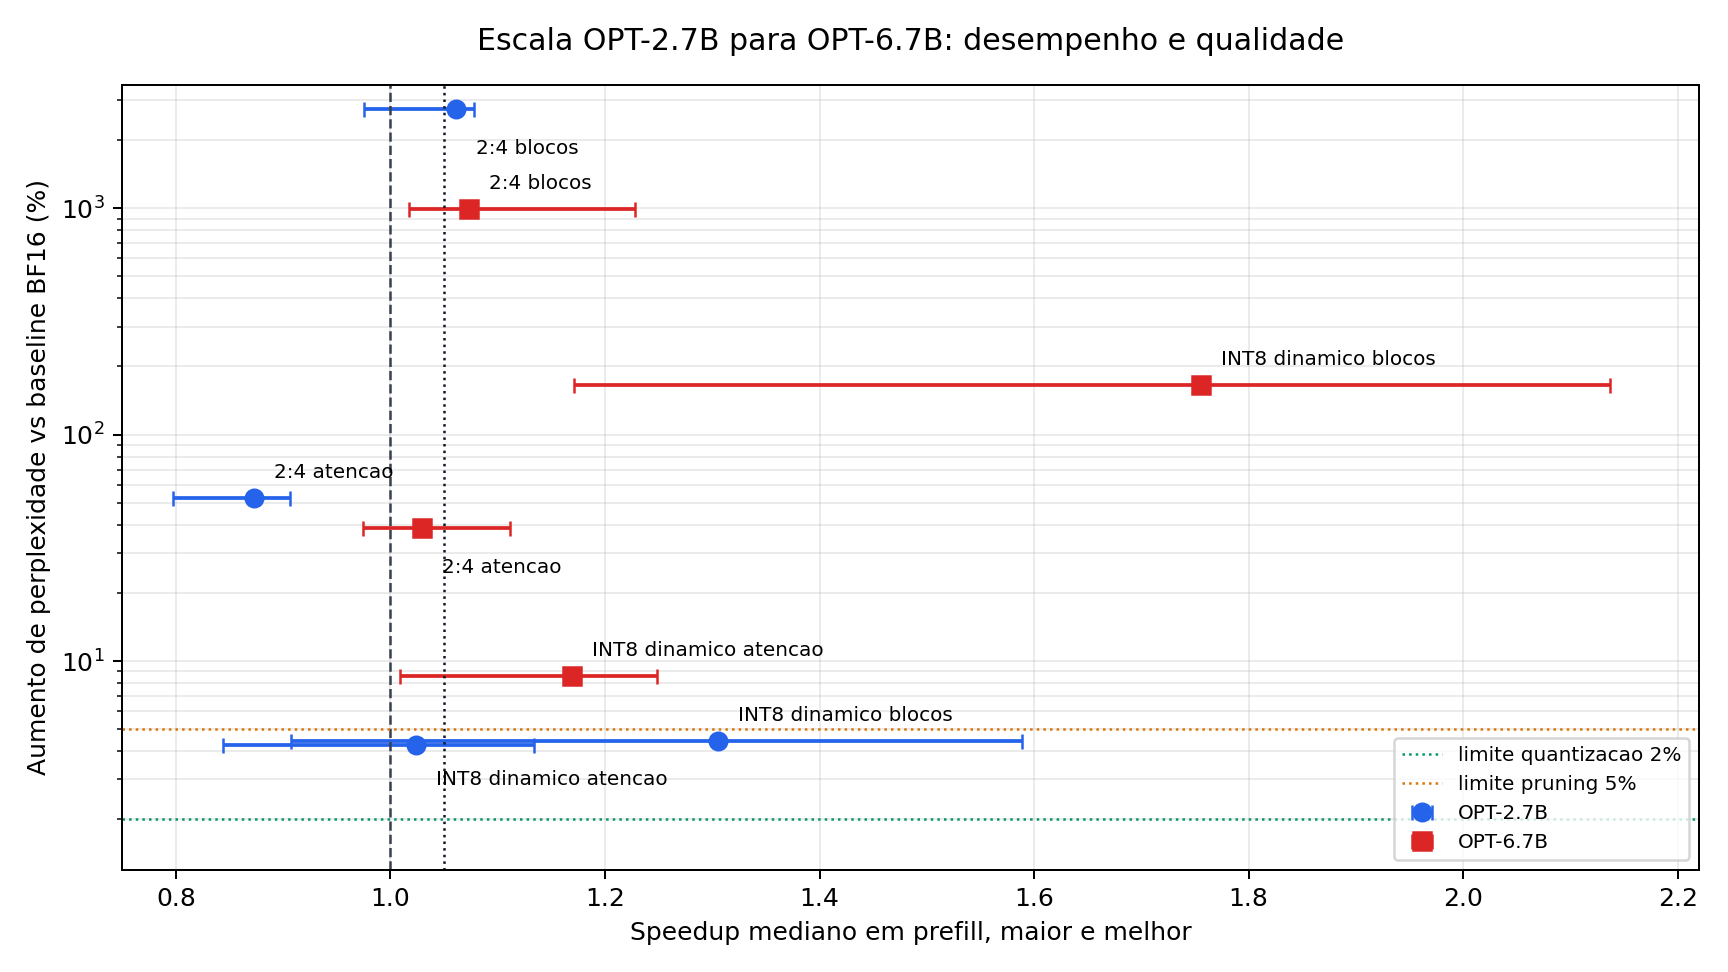
\includegraphics[width=0.88\textwidth]{figuras/opt_escala_2_7b_6_7b_tradeoff.png}
  \caption{Comparacao entre OPT-2.7B e OPT-6.7B no compromisso entre speedup de prefill e aumento de perplexidade.}
\end{figure}

\begin{figure}[H]
  \centering
  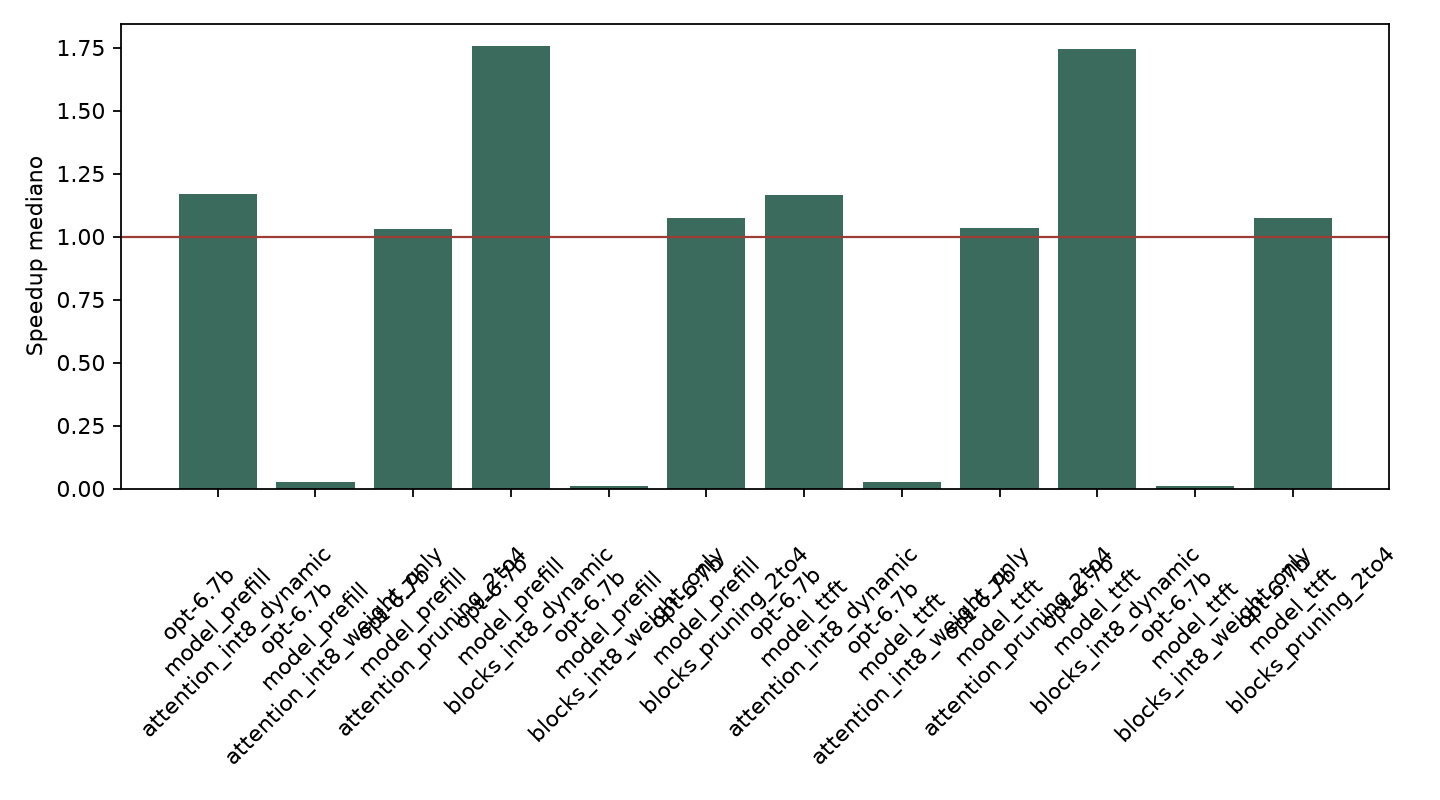
\includegraphics[width=0.88\textwidth]{figuras/opt_6_7b_speedup_prefill_decode.png}
  \caption{Speedup em prefill e TTFT na extensao OPT-6.7B.}
\end{figure}

\subsection{Sensibilidade e configuracoes hibridas}

A fase de sensibilidade avaliou INT8 dinamico por componente e regiao nos
modelos OPT-350M e OPT-1.3B. O objetivo foi verificar se atencao, MLP e regioes
do Transformer respondem de forma homogenea a quantizacao. Os resultados
indicaram sensibilidade heterogenea: configuracoes que preservavam componentes
mais sensiveis em BF16 podiam manter qualidade em modelos menores, enquanto
quantizacao ampla dos blocos tendia a aumentar a perplexidade.

Com base nessa leitura, foi executada uma etapa hibrida controlada. No
OPT-1.3B, configuracoes que preservaram a atencao sensivel conseguiram manter
qualidade. O controle envolvendo atencao final apresentou pior resultado. Os
finalistas hibridos com maior participacao de MLP quantizado tiveram medianas
de desempenho positivas, mas seus intervalos bootstrap de 95\% cruzaram 1,0x.
Portanto, nao houve speedup estatisticamente confirmado.

\begin{table}[H]
\centering
\caption{Finalistas hibridos no OPT-1.3B}
\resizebox{\textwidth}{!}{%
\begin{tabular}{lrrr}
\toprule
\textbf{Configuracao} & \textbf{Delta PPL} & \textbf{Speedup prefill} & \textbf{IC95 prefill} \\
\midrule
MLP todas, atencao BF16 & -1,098\% & 1,110 & [0,881; 1,309] \\
MLP todas, atencao 0--7 BF16 & -0,815\% & 1,131 & [0,872; 1,299] \\
MLP todas, atencao 0--15 BF16 & -0,370\% & 1,108 & [0,841; 1,310] \\
Atencao 0--15 quantizada & -0,102\% & 0,964 & [0,865; 0,990] \\
MLP 0--15, atencao BF16 & -1,506\% & 1,100 & [0,861; 1,178] \\
\bottomrule
\end{tabular}% 
}
\end{table}

No OPT-6.7B, todas as configuracoes hibridas testadas falharam em qualidade.
O aumento de perplexidade ficou aproximadamente entre +157\% e +207\%. Por
isso, o benchmark fisico dessas candidatas foi corretamente evitado: medir
latencia de configuracoes previamente descartadas por qualidade ampliaria custo
sem responder a pergunta principal.

\begin{table}[H]
\centering
\caption{Hibridos avaliados em qualidade no OPT-6.7B}
\resizebox{\textwidth}{!}{%
\begin{tabular}{lrrl}
\toprule
\textbf{Configuracao} & \textbf{PPL} & \textbf{Delta PPL} & \textbf{Decisao} \\
\midrule
Baseline BF16 & 15,346 & 0,0\% & referencia \\
INT8 dinamico em blocos & 40,675 & +165,052\% & descartado por qualidade \\
MLP todas, atencao BF16 & 47,151 & +207,254\% & descartado por qualidade \\
MLP todas, atencao 0--7 BF16 & 39,936 & +160,236\% & descartado por qualidade \\
MLP todas, atencao 0--15 BF16 & 39,481 & +157,271\% & descartado por qualidade \\
MLP 0--15, atencao BF16 & 45,589 & +197,073\% & descartado por qualidade \\
\bottomrule
\end{tabular}% 
}
\end{table}

A conclusao nao e que hibridos nao funcionam. Nas configuracoes avaliadas, a
seletividade por componente foi capaz de preservar qualidade no OPT-1.3B, mas
esse comportamento nao se transferiu para o OPT-6.7B. Portanto, a sensibilidade
observada em modelos menores nao se mostrou diretamente transferivel entre
escalas. Tambem nao foi demonstrada uma configuracao hibrida que combinasse
simultaneamente preservacao de qualidade e speedup confirmado no maior modelo
avaliado.

\subsection{Kernels confirmados}

O profiler registrou caminhos distintos para cada tecnica fisica. O INT8
weight-only acionou kernel de pesos empacotados, sendo classificado como
evidencia de armazenamento compacto. O INT8 dinamico registrou GEMM S8 via
CUTLASS, sustentando computa\c{c}\~ao inteira. O pruning 2:4 registrou sparse
GEMM por cuSPARSELt, sustentando representa\c{c}\~ao semiestruturada.

\begin{table}[H]
\centering
\caption{Classifica\c{c}\~ao dos caminhos fisicos}
\begin{tabular}{lll}
\toprule
\textbf{Cenario} & \textbf{Evidencia confirmada} & \textbf{Conclus\~ao permitida} \\
\midrule
INT8 fake & dequantiza\c{c}\~ao para FP32 & fidelidade numerica \\
INT8 weight-only & pesos empacotados INT8 & armazenamento compacto \\
INT8 dinamico & GEMM S8 no profiler & computa\c{c}\~ao inteira \\
Pruning 2:4 & sparse GEMM cuSPARSELt & caminho sparse fisico \\
\bottomrule
\end{tabular}
\end{table}

% -----------------------------------------------------------
\section{Discuss\~ao}
% -----------------------------------------------------------

Os resultados refor\c{c}am a necessidade de separar as camadas de evidencia. No
plano conceitual, a self-attention implementada manualmente e as vers\~oes de
frameworks consolidados chegaram ao mesmo resultado. No plano numerico, INT8
fake preservou melhor a saida que pruning denso. No plano fisico, tecnicas com
representa\c{c}\~ao real reduziram armazenamento e memoria, mas o custo de
convers\~ao, empacotamento, kernel e shape impediu ganho de latencia nas
opera\c{c}\~oes isoladas. Nos modelos OPT, a mesma tendencia de qualidade foi
observada parcialmente: INT8 preservou perplexidade melhor que pruning, enquanto
pruning degradou rapidamente conforme a sparsity aumentou. A extensao de escala
mostrou um resultado mais nuancado: em OPT-6.7B, INT8 dinamico e pruning 2:4
aplicados aos blocos tiveram speedup de prefill com intervalo acima de 1,0, mas
ambos ficaram fora dos limites de qualidade.

Isso nao significa que INT8 ou pruning 2:4 sejam tecnicas ineficazes de modo
geral. A conclus\~ao correta e mais estreita: na bateria principal, nao houve
speedup sustentado e aceitavel pelos criterios completos; na extensao OPT-6.7B,
houve speedup fisico em alguns caminhos, mas acompanhado de degradacao de
perplexidade. Essa leitura evita extrapolar benchmarks sinteticos, zeros
logicos ou speedup isolado sem verificar qualidade.

\subsection{Hipoteses finais}

\begin{longtable}{p{0.10\linewidth}p{0.22\linewidth}p{0.58\linewidth}}
\toprule
\textbf{Hip.} & \textbf{Classificacao} & \textbf{Evidencia resumida} \\
\midrule
H1 & sustentada & Reducao de precisao ou pesos nao implicou automaticamente reducao de latencia. \\
H2 & sustentada & Alteracao numerica, compressao fisica e aceleracao fisica apareceram como fenomenos distintos. \\
H3 & sustentada & Speedup dependeu de representacao, kernel e backend, nao apenas da tecnica nominal. \\
H4 & nao sustentada & O crossover fisico de operacoes isoladas nao encontrou ganho confirmado. \\
H5 & parcialmente sustentada & Workload e escala mudaram o comportamento, mas nao garantiram ganho util. \\
H6 & sustentada & Pruning denso revelou redundancia numerica sem produzir ganho fisico automatico. \\
H7 & parcialmente sustentada & 2:4 acionou sparse fisico, mas magnitude pruning degradou qualidade. \\
H8 & sustentada & Weight-only reduziu memoria/armazenamento e preservou qualidade, mas nao acelerou. \\
H9 & sustentada & Componentes e regioes tiveram sensibilidades diferentes a quantizacao. \\
H10 & nao sustentada & A politica observada em modelos menores nao transferiu ao OPT-6.7B. \\
H11 & nao sustentada & Nenhum hibrido combinou qualidade preservada e speedup confirmado no maior modelo. \\
H12 & parcialmente sustentada & Distribuicao e outliers influenciaram medicoes, sem reverter as conclusoes centrais. \\
\bottomrule
\end{longtable}

\subsection{Resultados negativos como evidencia}

Os resultados negativos delimitam o espaco experimental. A ausencia de
crossover confirmado nas operacoes isoladas mostra que kernels fisicos podem
ser anulados por overheads e shapes desfavoraveis. O weight-only muito lento
mostra que compressao de pesos nao e equivalente a aceleracao. O 2:4 por
magnitude mostra que sparsity fisica pode ser inviavel quando a selecao de
pesos degrada qualidade. O INT8 dinamico no OPT-6.7B mostra que escala pode
favorecer latencia, mas nao torna a configuracao util se a perplexidade cresce
fora dos limites. A falha dos hibridos no OPT-6.7B mostra que sensibilidade
observada em modelos menores nao deve ser transferida sem validacao.

\subsection{Respostas parciais as perguntas de pesquisa}

\begin{longtable}{p{0.13\linewidth}p{0.78\linewidth}}
\toprule
\textbf{Pergunta} & \textbf{Resposta ate esta vers\~ao} \\
\midrule
\RQ{1} & INT8 fake preservou melhor a saida que pruning em 100\% dos casos sinteticos pareados. \\
\RQ{2} & INT8 fisico reduziu armazenamento para cerca de 50\% e pruning 2:4 para cerca de 56\%; a memoria de pico tambem caiu. \\
\RQ{3} & Nenhum cenario fisico sustentou redu\c{c}\~ao de latencia; nos OPT, prefill e TTFT tambem nao cumpriram todos os criterios. \\
\RQ{4} & A separa\c{c}\~ao entre fidelidade, armazenamento, computa\c{c}\~ao inteira e sparse fisico foi confirmada. \\
\RQ{5} & As tendencias numericas persistiram entre cinco seeds, perfis e distribui\c{c}\~oes. \\
\RQ{6} & A degrada\c{c}\~ao aumentou conforme a sparsity passou de 10\% para 75\%. \\
\RQ{7} & Nos OPT, INT8 preservou melhor qualidade que pruning; a degradacao de pruning cresceu com sparsity; na extensao 6.7B o speedup apareceu, mas nao permaneceu aceitavel quando a qualidade foi considerada. \\
\RQ{8} & INT8 e 2:4 reduziram armazenamento e memoria com caminhos compativeis; apenas na extensao 6.7B alguns caminhos tiveram speedup fisico, sem cumprir simultaneamente os limites de qualidade. \\
\bottomrule
\end{longtable}

\subsection{Amea\c{c}as a validade}

As principais ameacas sao a limitacao da medicao de decode com KV cache no
compilador do PyTorch; a possibilidade de resultados diferentes em outros
shapes, GPUs ou bibliotecas; e a diferenca entre operacoes isoladas, prefill,
TTFT e execucao ponta a ponta de um modelo de linguagem. Alem disso, medicoes
de GPU podem sofrer interferencia de processos concorrentes, clocks dinamicos
e temperatura. Por isso, os runners exigem GPU ociosa antes da coleta final.

% -----------------------------------------------------------
\section{Limitacoes}
% -----------------------------------------------------------

O estudo foi executado em uma unica GPU principal, uma RTX 4070 Ti SUPER, e em
uma unica familia de modelos, OPT. O dataset de qualidade foi relativamente
estreito: WikiText-2 com 64 janelas de 512 tokens. A avaliacao de geracao usou
20 prompts locais e decoding greedy, sem multiplas seeds independentes de
dataset ou prompts. Os clocks e estados de energia da GPU nao foram fixados,
embora o protocolo tenha usado GPU ociosa, warm-up, sincronizacao CUDA,
repeticoes e bootstrap para reduzir ruido.

O campo historico \texttt{model\_ttft} mede, na pratica,
\texttt{prefill\_to\_first\_logit}; nao e TTFT completo de sistema com
tokenizacao, fila, streaming e overhead de servico. A confirmacao de kernels e
mais forte nos caminhos em que o profiler registrou explicitamente os
operadores esperados. O backend weight-only avaliado nao representa todos os
backends possiveis. O pruning 2:4 atual usa selecao simples por magnitude. Por
fim, o espaco hibrido foi propositalmente pequeno e nao deve ser lido como busca
exaustiva.

% -----------------------------------------------------------
\section{Trabalhos futuros}
% -----------------------------------------------------------

Os resultados sugerem trabalhos futuros sem transforma-los em pendencias
obrigatorias desta iniciacao cientifica. O primeiro caminho e avaliar kernels
weight-only mais especializados, mantendo a distincao entre compressao e
latencia. O segundo e substituir a selecao simples por magnitude no 2:4 por uma
estrategia post-training informada por ativacoes, como Wanda
\cite{sun2024wanda}; SparseGPT \cite{frantar2023sparsegpt} tambem e relevante,
mas tem custo e complexidade maiores. Outras continuacoes naturais incluem
quantizacao com tratamento explicito de outliers, outras GPUs, outras familias
de LLMs, politicas sensiveis a camada e calibracao hibrida mais sofisticada.

Para o fechamento atual, Wanda e classificada como util mas opcional. Ela
ajudaria a separar se a falha de qualidade do 2:4 vem do formato sparse ou da
selecao ingenua de pesos, mas a tese central da pesquisa ja esta sustentada
pelos dados existentes.

% -----------------------------------------------------------
\section{Conclus\~ao}
% -----------------------------------------------------------

O estudo validou conceitualmente a implementacao de self-attention e consolidou
uma cadeia experimental que vai de operacoes deterministicas ate modelos OPT
pre-treinados. A evidencia sintetica mostra que INT8 fake preserva melhor a
saida que pruning por magnitude. A evidencia fisica mostra que representacoes
compactas reduzem armazenamento e memoria, mas nao garantem latencia menor. A
avaliacao em OPT mostra que speedup pode aparecer em escala maior, mas pode ser
anulado cientificamente por degradacao de qualidade.

A contribuicao principal e metodologica e experimental: o trabalho separa
alteracao numerica, compressao fisica e aceleracao fisica, e mostra que cada
uma precisa ser medida com instrumentos diferentes. Weight-only preservou
qualidade e comprimiu memoria, mas nao acelerou no backend avaliado. INT8
dinamico acelerou alguns caminhos do OPT-6.7B, mas com perplexidade fora dos
limites. 2:4 confirmou sparse fisico, mas a selecao por magnitude degradou
qualidade. Hibridos preservaram qualidade no OPT-1.3B, mas nao apresentaram
speedup confirmado e nao transferiram essa qualidade ao OPT-6.7B.

Assim, os dados atuais sao suficientes para encerrar a iniciacao cientifica: a
pesquisa responde, com evidencia rastreavel, que reduzir bits ou pesos nao
implica automaticamente acelerar inferencia. O beneficio final depende de
representacao, kernel, workload, qualidade e escala.

% -----------------------------------------------------------
\printbibliography[title={Refer\^encias}]

\end{document}
